\documentclass[11pt,oneside]{article}
\usepackage[T1]{fontenc}
\usepackage[utf8]{inputenc}
% \usepackage{lmodern}
%\usepackage[adobe-utopia,uppercase=upright,greeklowercase=upright]{mathdesign}
\usepackage[adobe-utopia]{mathdesign}
%\usepackage{minionpro}
% \usepackage{pifont}
% \usepackage{amssymb}
\usepackage{amsmath}
\usepackage[francais]{babel}
% \usepackage[francais]{varioref}
\usepackage[dvips]{graphicx}

\usepackage{framed}
\usepackage[normalem]{ulem}
\usepackage{fancyhdr}
\usepackage{titlesec}
\usepackage{vmargin}
\usepackage{longtable}

\usepackage{ifthen}


%\usepackage{epsfig}
\usepackage{subfig}

\usepackage{multirow}
\usepackage{multicol} % Portions de texte en colonnes
\usepackage{flafter}%floatants après la référence



\usepackage{color}
\usepackage{colortbl}


\definecolor{gris25}{gray}{0.75}
\definecolor{bleu}{RGB}{18,33,98}
\definecolor{bleuf}{RGB}{42,94,171}
\definecolor{bleuc}{RGB}{231,239,247}
\definecolor{rougef}{RGB}{185,18,27}
\definecolor{rougec}{RGB}{255,230,231}
\definecolor{vertf}{RGB}{103,126,82}
\definecolor{vertc}{RGB}{220,255,191}
\definecolor{violetf}{RGB}{112,48,160}
\definecolor{violetc}{RGB}{230,224,236}

\newenvironment{sci}[1][\hsize]%
{%
    \def\FrameCommand%
    {%
%\rotatebox{90}{\textit{\textsf{Scilab}}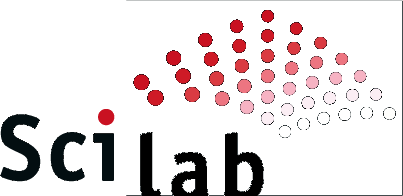
\includegraphics[height=.8cm]{png/logo_scilab}} 
\rotatebox{90}{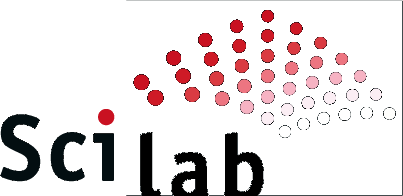
\includegraphics[height=.6cm]{png/logo_scilab}} 
        {\color{violetf}\vrule width 3pt}%
        \hspace{0pt}%must no space.
        \fboxsep=\FrameSep\colorbox{violetc}%
    }%
    \MakeFramed{\hsize #1 \advance\hsize-\width\FrameRestore}%
}%
{\endMakeFramed}%

\newenvironment{pseudo}[1][\hsize]%
{%
    \def\FrameCommand%
    {%
\rotatebox{90}{\textit{\textsf{Pseudo Code}}} 
        {\color{violetf}\vrule width 3pt}%
        \hspace{0pt}%must no space.
        \fboxsep=\FrameSep\colorbox{violetc}%
    }%
    \MakeFramed{\hsize #1 \advance\hsize-\width\FrameRestore}%
}%
{\endMakeFramed}%

\newenvironment{py}[1][\hsize]%
{%
    \def\FrameCommand%
    {%
%\rotatebox{90}{\textit{\textsf{Python}}} 
\rotatebox{90}{
\includegraphics[height=.6cm]{png/logo_python}} 
        {\color{violetf}\vrule width 3pt}%
        \hspace{0pt}%must no space.
        \fboxsep=\FrameSep\colorbox{violetc}%
    }%
    \MakeFramed{\hsize #1 \advance\hsize-\width\FrameRestore}%
}%
{\endMakeFramed}%


\newenvironment{corrige}[1][\hsize]%
{%
    \def\FrameCommand
    {%
\rotatebox{90}{\textit{\textsf{Correction}}} 
        {\color{violetf}\vrule width 3pt}%
        \hspace{0pt}%must no space.
        \fboxsep=\FrameSep\colorbox{violetc}%
    }%
    \MakeFramed{\hsize#1\advance\hsize-\width\FrameRestore}%
}%
{\endMakeFramed}%



\newenvironment{rem}[1][\hsize]%
{%
    \def\FrameCommand
    {%
\rotatebox{90}{\textit{\textsf{Remarque}}} 
        {\color{bleuf}\vrule width 3pt}%
        \hspace{0pt}%must no space.
        \fboxsep=\FrameSep\colorbox{bleuc}%
    }%
    \MakeFramed{\hsize#1\advance\hsize-\width\FrameRestore}%
}%
{\endMakeFramed}%


\newenvironment{savoir}[1][\hsize]%
{%
    \def\FrameCommand
    {%
\rotatebox{90}{\textit{\textsf{Savoir}}} 
        {\color{bleuf}\vrule width 3pt}%
        \hspace{0pt}%must no space.
        \fboxsep=\FrameSep\colorbox{bleuc}%
    }%
    \MakeFramed{\hsize#1\advance\hsize-\width\FrameRestore}%
}%
{\endMakeFramed}%

\newenvironment{prob}[1][\hsize]%
{%
    \def\FrameCommand%
    {%
\rotatebox{90}{\textit{\textsf{ Problématique}}} 
        {\color{rougef}\vrule width 3pt}%
        \hspace{0pt}%must no space.
        \fboxsep=\FrameSep\colorbox{rougec}%
    }%
    \MakeFramed{\hsize#1\advance\hsize-\width\FrameRestore}%
}%
{\endMakeFramed}%

\newenvironment{obj}[1][\hsize]%
{%
    \def\FrameCommand%
    {%
\rotatebox{90}{\textit{\textsf{Objectifs}}} 
        {\color{rougef}\vrule width 3pt}%
        \hspace{0pt}%must no space.
        \fboxsep=\FrameSep\colorbox{rougec}%
    }%
    \MakeFramed{\hsize#1\advance\hsize-\width\FrameRestore}%
}%
{\endMakeFramed}%

\newenvironment{defi}[1][\hsize]%
{%
    \def\FrameCommand%
    {%
\rotatebox{90}{\textit{\textsf{Définition\\}}} 
        {\color{bleuf}\vrule width 3pt}%
        \hspace{0pt}%must no space.
        \fboxsep=\FrameSep\colorbox{bleuc}%
    }%
    \MakeFramed{\hsize#1\advance\hsize-\width\FrameRestore}%
}%
{\endMakeFramed}%


\newenvironment{demo}[1][\hsize]%
{%
    \def\FrameCommand%
    {%
\rotatebox{90}{\textit{\textsf{Démonstration\\}}} 
        {\color{bleuf}\vrule width 3pt}%
        \hspace{0pt}%must no space.
        \fboxsep=\FrameSep\colorbox{bleuc}%
    }%
    \MakeFramed{\hsize#1\advance\hsize-\width\FrameRestore}%
}%
{\endMakeFramed}%


\newenvironment{hypo}[1][\hsize]%
{%
    \def\FrameCommand%
    {%
\rotatebox{90}{\textit{\textsf{Hypothèse\\}}} 
        {\color{bleuf}\vrule width 3pt}%
        \hspace{0pt}%must no space.
        \fboxsep=\FrameSep\colorbox{bleuc}%
    }%
    \MakeFramed{\hsize#1\advance\hsize-\width\FrameRestore}%
}%
{\endMakeFramed}%


\newenvironment{prop}[1][\hsize]%
{%
    \def\FrameCommand%
    {%
\rotatebox{90}{\textit{\textsf{Propriété\\}}} 
        {\color{bleuf}\vrule width 3pt}%
        \hspace{0pt}%must no space.
        \fboxsep=\FrameSep\colorbox{bleuc}%
    }%
    \MakeFramed{\hsize#1\advance\hsize-\width\FrameRestore}%
}%
{\endMakeFramed}%

\newenvironment{props}[1][\hsize]%
{%
    \def\FrameCommand%
    {%
\rotatebox{90}{\textit{\textsf{Propriétés\\}}} 
        {\color{bleuf}\vrule width 3pt}%
        \hspace{0pt}%must no space.
        \fboxsep=\FrameSep\colorbox{bleuc}%
    }%
    \MakeFramed{\hsize#1\advance\hsize-\width\FrameRestore}%
}%
{\endMakeFramed}%

\newenvironment{exemple}[1][\hsize]%
{%
    \def\FrameCommand%
    {%
\rotatebox{90}{\textit{\textsf{Exemple\\}}} 
        {\color{vertf}\vrule width 3pt}%
        \hspace{0pt}%must no space.
        \fboxsep=\FrameSep\colorbox{vertc}%
    }%
    \MakeFramed{\hsize#1\advance\hsize-\width\FrameRestore}%
}%
{\endMakeFramed}%

\newenvironment{resultat}[1][\hsize]%
{%
    \def\FrameCommand%
    {%
\rotatebox{90}{\textit{\textsf{Résultat\\}}} 
        {\color{rougef}\vrule width 3pt}%
        \hspace{0pt}%must no space.
        \fboxsep=\FrameSep\colorbox{rougec}%
    }%
    \MakeFramed{\hsize#1\advance\hsize-\width\FrameRestore}%
}%
{\endMakeFramed}%

\newenvironment{methode}[1][\hsize]%
{%
    \def\FrameCommand%
    {%
\rotatebox{90}{\textit{\textsf{Méthode\\}}} 
        {\color{rougef}\vrule width 3pt}%
        \hspace{0pt}%must no space.
        \fboxsep=\FrameSep\colorbox{rougec}%
    }%
    \MakeFramed{\hsize#1\advance\hsize-\width\FrameRestore}%
}%
{\endMakeFramed}%

\newenvironment{theo}[1][\hsize]%
{%
    \def\FrameCommand%
    {%
\rotatebox{90}{\textit{\textsf{Théorème\\}}} 
        {\color{rougef}\vrule width 3pt}%
        \hspace{0pt}%must no space.
        \fboxsep=\FrameSep\colorbox{rougec}%
    }%
    \MakeFramed{\hsize#1\advance\hsize-\width\FrameRestore}%
}%
{\endMakeFramed}%

\newenvironment{warn}[1][\hsize]%
{%
    \def\FrameCommand%
    {%
\rotatebox{90}{\textit{\textsf{Attention\\}}} 
        {\color{rougef}\vrule width 3pt}%
        \hspace{0pt}%must no space.
        \fboxsep=\FrameSep\colorbox{rougec}%
    }%
    \MakeFramed{\hsize#1\advance\hsize-\width\FrameRestore}%
}%
{\endMakeFramed}%

% \usepackage{pstricks}
%\usepackage{minitoc}
% \setcounter{minitocdepth}{4}

\setcounter{tocdepth}{2}

% \mtcselectlanguage{french} 

%\usepackage{draftcopy}% "Brouillon"
% \usepackage{floatflt}
\usepackage{psfrag}
%\usepackage{listings} % Permet d'insérer du code de programmation
\renewcommand{\baselinestretch}{1.2}

% Changer la numérotation des figures :
% ------------------------------------
% \makeatletter
% \renewcommand{\thefigure}{\ifnum \c@section>\z@ \thesection.\fi
%  \@arabic\c@figure}
% \@addtoreset{figure}{section}
% \makeatother
 


%%%%%%%%%%%%
% Définition des vecteurs %
%%%%%%%%%%%%
 \newcommand{\vect}[1]{\overrightarrow{#1}}

%%%%%%%%%%%%
% Définition des torseusr %
%%%%%%%%%%%%

 \newcommand{\torseur}[1]{%
\left\{{#1}\right\}
}

\newcommand{\torseurcin}[3]{%
\left\{\mathcal{#1} \left(#2/#3 \right) \right\}
}

\newcommand{\torseurstat}[3]{%
\left\{\mathcal{#1} \left(#2\rightarrow #3 \right) \right\}
}

 \newcommand{\torseurc}[8]{%
%\left\{#1 \right\}=
\left\{
{#1}
\right\}
 = 
\left\{%
\begin{array}{cc}%
{#2} & {#5}\\%
{#3} & {#6}\\%
{#4} & {#7}\\%
\end{array}%
\right\}_{#8}%
}

 \newcommand{\torseurcol}[7]{
\left\{%
\begin{array}{cc}%
{#1} & {#4}\\%
{#2} & {#5}\\%
{#3} & {#6}\\%
\end{array}%
\right\}_{#7}%
}

 \newcommand{\torseurl}[3]{%
%\left\{\mathcal{#1}\right\}_{#2}=%
\left\{%
\begin{array}{l}%
{#1} \\%
{#2} %
\end{array}%
\right\}_{#3}%
}

 \newcommand{\vectv}[3]{%
\vect{V\left( {#1} \in {#2}/{#3}\right)}
}


\newcommand{\vectf}[2]{%
\vect{R\left( {#1} \rightarrow {#2}\right)}
}

\newcommand{\vectm}[3]{%
\vect{\mathcal{M}\left( {#1}, {#2} \rightarrow {#3}\right)}
}


 \newcommand{\vectg}[3]{%
\vect{\Gamma \left( {#1} \in {#2}/{#3}\right)}
}

 \newcommand{\vecto}[2]{%
\vect{\Omega\left( {#1}/{#2}\right)}
}
% }$$\left\{\mathcal{#1} \right\}_{#2} =%
% \left\{%
% \begin{array}{c}%
%  #3 \\%
%  #4 %
% \end{array}%
% \right\}_{#5}}

%  ------------------------------------------
% | Modification du formatage des sections : | 
%  ------------------------------------------

% Grands titres :
% ---------------

\newcommand{\titre}[1]{%
\begin{center}
      \bigskip
      \rule{\textwidth}{1pt}
      \par\vspace{0.1cm}
      
      \textbf{\large #1}
      \par\rule{\textwidth}{1pt}
    \end{center}
    \bigskip
  }

% Supprime le numéro du chapitre dans la numérotation des sections:
% -----------------------------------------------------------------
\makeatletter
\renewcommand{\thesection}{\@arabic\c@section}
\makeatother


% \titleformat{\chapter}[display]
% {\normalfont\Large\filcenter}
% {}
% {1pc}
% {\titlerule[1pt]
%   \vspace{1pc}%
%   \Huge}[\vspace{1ex}%
% \titlerule]


%%%% Chapitres Comme PY Pechard %%%%%%%%%
% numéro du chapitre
\DeclareFixedFont{\chapnumfont}{OT1}{phv}{b}{n}{80pt}
% pour le mot « Chapitre »
\DeclareFixedFont{\chapchapfont}{OT1}{phv}{m}{it}{40pt}
% pour le titre
\DeclareFixedFont{\chaptitfont}{T1}{phv}{b}{n}{25pt}

\definecolor{gris}{gray}{0.75}
\titleformat{\chapter}[display]%
	{\sffamily}%
	{\filleft\chapchapfont\color{gris}\chaptertitlename\
	\\
	\vspace{12pt}
	\chapnumfont\thechapter}%
	{16pt}%
	{\filleft\chaptitfont}%
	[\vspace{6pt}\titlerule\titlerule\titlerule]

%%%%  Fin Chapitres Comme PY Pechard %%%%%%%%%


% Section, subsection, subsubsection sans serifs :
% % ----------------------------------------------

% \makeatletter
% \renewcommand{\section}{\@startsection{section}{0}{0mm}%
% {\baselineskip}{.3\baselineskip}%
% {\normalfont\sffamily\Large\textbf}}%
% \makeatother

\makeatletter
\renewcommand{\@seccntformat}[1]{{\textcolor{bleu}{\csname
the#1\endcsname}\hspace{0.5em}}}
\makeatother

\makeatletter
\renewcommand{\section}{\@startsection{section}{1}{\z@}%
                       {-4ex \@plus -1ex \@minus -.4ex}%
                       {1ex \@plus.2ex }%
                       {\normalfont\Large\sffamily\bfseries}}%
\makeatother
 
\makeatletter
\renewcommand{\subsection}{\@startsection {subsection}{2}{\z@}
                          {-3ex \@plus -0.1ex \@minus -.4ex}%
                          {0.5ex \@plus.2ex }%
                          {\normalfont\large\sffamily\bfseries}}
\makeatother
 
\makeatletter
\renewcommand{\subsubsection}{\@startsection {subsubsection}{3}{\z@}
                          {-2ex \@plus -0.1ex \@minus -.2ex}%
                          {0.2ex \@plus.2ex }%
                          {\normalfont\large\sffamily\bfseries}}
\makeatother
 
\makeatletter             
\renewcommand{\paragraph}{\@startsection{paragraph}{4}{\z@}%
                                    {-2ex \@plus-.2ex \@minus .2ex}%
                                    {0.1ex}%               
{\normalfont\sffamily\bfseries}}
\makeatother
 

\makeatletter             
\renewcommand{\subparagraph}{\@startsection{subparagraph}{5}{\z@}%
                                    {-2ex \@plus-.2ex \@minus .2ex}%
                                    {0.1ex}%               
{\normalfont\bfseries Question }}
\makeatother

\renewcommand{\thesubparagraph}{\arabic{subparagraph}} 
\makeatletter

\setcounter{secnumdepth}{5}
%\renewcommand{\subparagraph}{\@startsection{subparagraph}{5}{\z@}%
%                                       {-2ex \@plus-.1ex \@minus .2ex}%
%                                       {0.1ex}%
%				    {\normalfont\normalsize\sffamily\bfseries}}
%\makeatletter
% \makeatletter
% \renewcommand{\subsection}{\@startsection{subsection}{1}{2mm}%
% {\baselineskip}{.3\baselineskip}%
% {\normalfont\sffamily\large\textbf}}%
% \makeatother
% 
% \makeatletter
% \renewcommand{\subsubsection}{\@startsection{subsubsection}{2}{4mm}%
% {\baselineskip}{.15\baselineskip}%
% {\normalfont\sffamily\large\textbf}}%
% \makeatother
% 
% \makeatletter
% \renewcommand{\paragraph}{\@startsection{paragraph}{3}{6mm}%
% {\baselineskip}{.15\baselineskip}%
% {\normalfont\sffamily\large\textbf}}%
% \makeatother
 



%  --------
% | Marges |
%  --------


% \setmarginsrb{2.5cm}{1.5cm}{2.5cm}{2cm}{1cm}{1cm}{1cm}{1cm}
\setmarginsrb{1.5cm}{1cm}{1cm}{1.5cm}{1cm}{1cm}{1cm}{1cm}

% Changer les marges localement :
% -----------------------------
\newenvironment{changemargin}[2]{\begin{list}{}{%
\setlength{\topsep}{0pt}%
\setlength{\leftmargin}{0pt}%
\setlength{\rightmargin}{0pt}%
\setlength{\listparindent}{\parindent}%
\setlength{\itemindent}{\parindent}%
\setlength{\parsep}{0pt plus 1pt}%
\addtolength{\leftmargin}{#1}%
\addtolength{\rightmargin}{#2}%
}\item }{\end{list}}



\usepackage{pst-solides3d}
\usepackage{titletoc}
\titlecontents{chapter}[+3pc]
  {\addvspace{10pt}\sffamily\bfseries}
{\contentslabel[{\pscirclebox[fillstyle=solid,fillcolor=gray!25,
linecolor=gray!25,framesep=4pt]{\textcolor{white}{\thecontentslabel}}}]{2.5pc}}
  {}
  {\dotfill \normalfont\thecontentspage\ }

\titlecontents{section}[3pc]
  {\addvspace{2pt}\sffamily}
  {\contentslabel[\thecontentslabel]{1.8pc}}
  {}
  {\dotfill \normalfont\thecontentspage\ }

\titlecontents{subsection}[5pc]
  {\addvspace{2pt}\sffamily}
  {\contentslabel[\thecontentslabel]{1.8pc}}
  {}
  {\dotfill \normalfont\thecontentspage\ }

\titlecontents{subsubsection}[8pc]
  {\addvspace{2pt}\sffamily}
  {\contentslabel[\thecontentslabel]{3pc}}
  {}
  {\dotfill \normalfont\thecontentspage\ }
%{\;\titlerule\;\normalfont\thecontentspage\ }

\titlecontents{paragraph}[9pc]
  {\addvspace{2pt}\sffamily}
  {\contentslabel[\thecontentslabel]{3.5pc}}
  {}
  {\dotfill \normalfont\thecontentspage\ }




\usepackage[%
    pdftitle={SLCI -- Devoir Maison 2},
    pdfauthor={Xavier Pessoles},
    colorlinks=true,
    linkcolor=blue,
    citecolor=magenta]{hyperref}



% \makeatletter \let\ps@plain\ps@empty \makeatother
%% DEBUT DU DOCUMENT
%% =================
\sloppy
\hyphenpenalty 10000

\newcommand{\Pointilles}[1][3]{%
\multido{}{#1}{\makebox[\linewidth]{\dotfill}\\[\parskip]
}}


\begin{document}


\newboolean{prof}
\setboolean{prof}{false}
%------------- En tetes et Pieds de Pages ------------
\pagestyle{fancy}
\renewcommand{\headrulewidth}{0pt}

\fancyhead{}
\fancyhead[L]{%
\noindent\noindent\begin{minipage}[c]{2.6cm}
%Lycée Rouvière PTSI

\includegraphics[width=2cm]{png/logo_ptsi.png}%
\end{minipage}
}

\fancyhead[C]{\rule{12cm}{.5pt}}

\fancyhead[R]{%
\begin{minipage}[c]{3cm}
\begin{flushright}
\footnotesize{\textit{\textsf{Sciences Industrielles\\ de l'Ingénieur}}}%
\end{flushright}
\end{minipage}
}

\renewcommand{\footrulewidth}{0.2pt}

\fancyfoot[C]{\footnotesize{\bfseries \thepage}}
\fancyfoot[L]{\footnotesize{2013 -- 2014} \\ David \textsc{Violeau}}
\ifthenelse{\boolean{prof}}{%
\fancyfoot[R]{\footnotesize{CI 2 : SLCI } \\ \footnotesize{DM 2 -- Corrigé}}
}{%
\fancyfoot[R]{\footnotesize{CI 2 : SLCI} \\ \footnotesize{DM 2 -- Sujet}}
}


%\begin{center}
%\textit{Centre d'intérêt}
%\end{center}



\begin{center}
 \Large\textsc{CI 2 -- SLCI : Étude du comportement des Systèmes Linéaires Continus Invariants}
\end{center}
%
%\begin{center}
% \large\textsc{Chapitre 2 -- Modélisation des Systèmes Linéaires Continus Invariants}
%
% \large\textsc{Transformée de Laplace} 
%\end{center}

\begin{center}
\textsc{Devoir Maison 2 -- Système de freinage d'un TGV DUPLEX} 
\ifthenelse{\boolean{prof}}{

\textbf{\textsc{Éléments de corrigé}}}{}
\end{center}

\ifthenelse{\boolean{prof}}{
\begin{flushright}
\textit{D'après ressources de David Violeau.} 
\end{flushright}
\vspace{.5cm}
}{
}

\vspace{1cm}



\subsection*{Présentation}
\ifthenelse{\boolean{prof}}{}{
\vspace{.5cm}
\noindent\begin{minipage}[c]{.5\linewidth}
\indent Pour satisfaire la croissance de la demande de ses usagers, la SNCF a besoin
d’augmenter le nombre des passagers transportés sur les lignes TGV existantes. 
Pour y répondre, les constructeurs ont réalisé des voitures à deux étages, les
TGV duplex, qui permettent d’accueillir plus de passagers par
rame.

 Parallèlement, ils souhaitent en augmenter la vitesse et la fréquence
d’utilisation. Mais ces solutions sont limitées par la distance d’arrêt car il ne
faut pas percuter la rame précédente, brutalement immobilisée. 

\end{minipage}\hfill
\begin{minipage}[c]{.47\linewidth}
\begin{center}
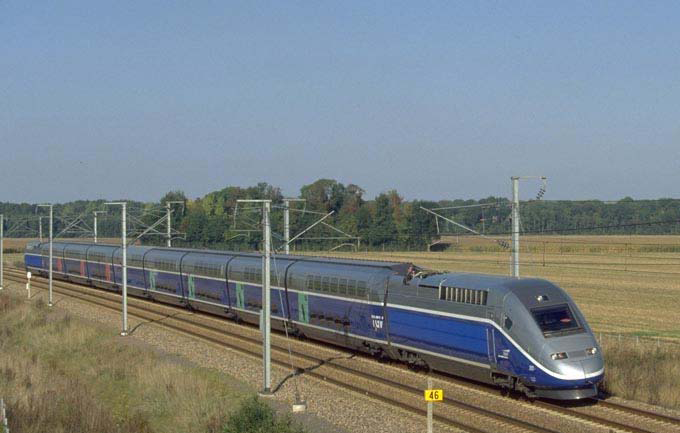
\includegraphics[width=.95\textwidth]{png/rame}
\end{center}
\end{minipage}

\vspace{.5cm}
Cette évidente condition de sécurité place les dispositifs de freinage au c\oe{}ur des travaux
d'innovation des ingénieurs. L’objet de cette étude est l’analyse du système
de freinage mécanique à énergie pneumatique, installé sur les TGV Duplex
vis-à-vis du critère de la validation partielle de l’une des prestations attendues :
« le conducteur actionne le système de
freinage pour ne pas percuter une autre
rame ».

%\begin{center}
%
%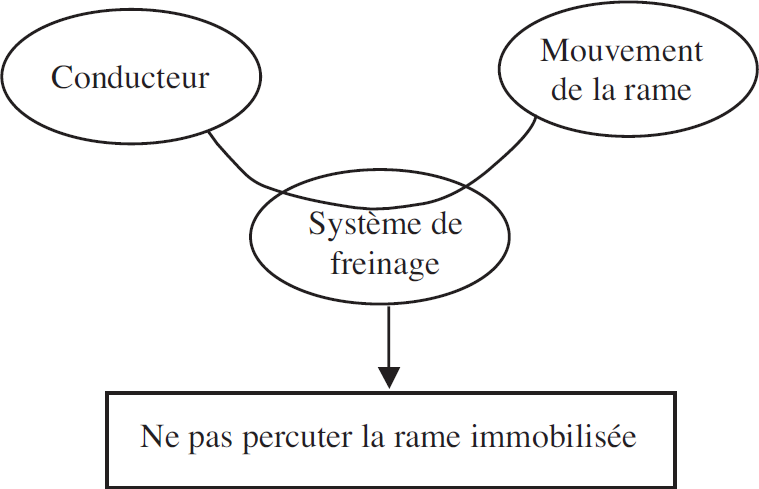
\includegraphics[width=.4\textwidth]{png/beteacorne} 
%\begin{tabular}{|c|c|}
%\hline
%Critère & Valeur \\
%\hline
%Distance d'arrêt de la rame & $da \leq 2500m$\\
%\hline
%\end{tabular}
%
%\end{center}

Une rame de TGV est composée de deux motrices et de huit voitures.
La liaison avec les rails est assurée par bogies. Quatre d’entre eux, implantés
sous les motrices, sont moteurs, les neuf autres, qualifiés de porteurs, sont positionnés
entre deux voitures.

\begin{center}
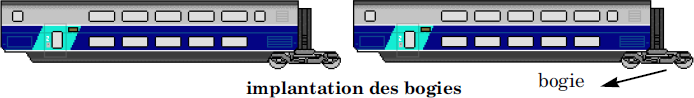
\includegraphics[width=.8\textwidth]{png/bogies.png}
\end{center}

\begin{minipage}[c]{.6\linewidth}
Pour l’étude proposée tous les bogies ont le même comportement. Un bogie porteur, dont une photo est donnée ci-contre, est un chariot à deux essieux et quatre roues. Il supporte en sa partie supérieure l’une des extrémités de la voiture et permet de suivre les courbes de la voie. Chacune des roues est équipée d’un système de freinage à disques et contribue à l’arrêt de la voiture.
Dans cette étude, la masse de la rame, estimée à $420\,000\,kg$, est supposée également répartie sur chacune des roues. Cette hypothèse permet de limiter l’étude à une roue, ses deux disques et les composants associés.
\end{minipage}\hfill
\begin{minipage}[c]{.35\linewidth}
\begin{center}
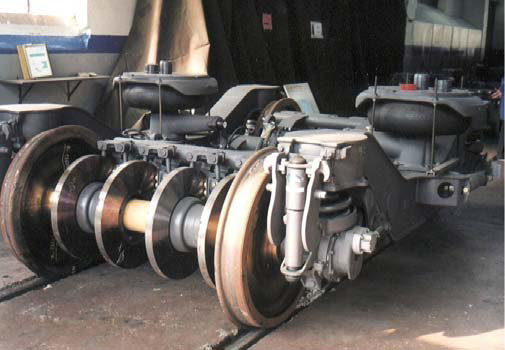
\includegraphics[width=.95\textwidth]{png/bogie_porteur.png}
\end{center}
\end{minipage}

%La prestation attendue est réalisée pendant la phase de vie « arrêt d’urgence »
%dont la caractérisation partielle des principales fonctions de service est donnée
%ci-dessous :
%
%\begin{center}
%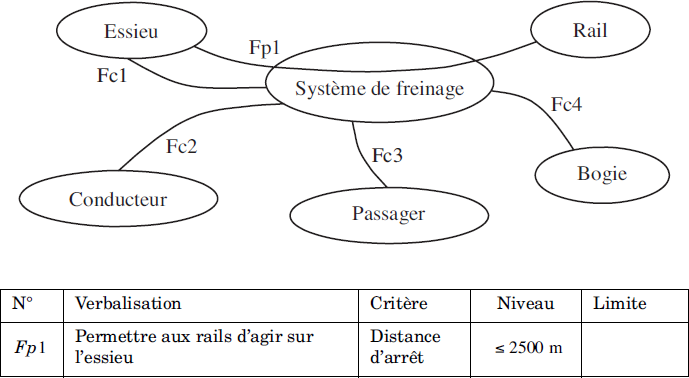
\includegraphics[width=.8\textwidth]{png/pieuvre.png}
%\end{center}
%
}
\subsection*{Dispositif d’anti-enrayage}
\ifthenelse{\boolean{prof}}{}{
Parmi les solutions utilisées pour le freinage des trains, on utilise un dispositif de frein à disque. L'inconvénient de ce type de système est le blocage des roues appelé aussi enrayage. Lors du blocage des roues, la distance de freinage peut être considérablement agrandi. Dans certains cas ce blocage peut mener au déraillement du train.

On appelle $V_T$ ($V_T>0$) la vitesse de translation du train et $V_R$ ($V_R>0$) l'opposée de la vitesse du point de contact appartenant à la roue par rapport au bogie. On appelle $\nu$ le glissement relatif au contact entre la roue et le rail. On a $\nu = 1-\dfrac{V_R}{V_T}$. Ainsi en cas de blocage des roues $\nu=1$ et $\nu=0$ lorsqu'il n'y a aucune action de freinage.

%L’objectif est d'étudier de la loi de commande du dispositif d’anti-enrayage et plus précisément le calcul du correcteur de la boucle de régulation.

La réalisation de la régulation de glissement ne peut être effectuée directement, en particulier la seule mesure généralement disponible est celle de la vitesse $V_R$, aussi la vitesse $V_T$ est obtenue par estimation. En « pratique », la mise en place de la chaîne de régulation du dispositif d'anti-enrayage du système de freinage est conçue de la façon suivante :
\begin{itemize}
\item elle est réalisée au travers de l'asservissement des vitesses des roues à une consigne de référence obtenue à partir de $V_T$;
\item la commande de l'actionneur est non linéaire, de type tout ou rien;
\item les algorithmes implémentés visent à optimiser le point de fonctionnement
en vue de minimiser la distance de freinage.
\end{itemize}
Cependant, dans le cadre de cette étude, on supposera que :
\begin{itemize}
\item les vitesses $V_R$ et $V_T$ sont directement accessibles à la mesure, éventuellement
entachées d’une erreur ;
\item la régulation peut se ramener directement à celle du glissement ;
\item le comportement de l’actionneur et de sa « commande rapprochée » est modélisé
par une fonction de transfert linéaire correspondant à un comportement
« moyen ».
\end{itemize}
On donne un extrait du cahier des charges associé au dispositif d'anti-enrayage.
\begin{center}
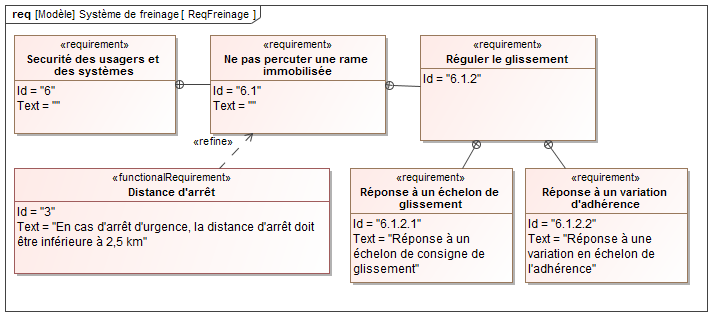
\includegraphics[width=.95\linewidth]{png/ReqFreinage}
\end{center}
}

\begin{obj}
\begin{minipage}[c]{.47\linewidth}
L'objectif est de valider les critères du cahier des charges ci-contre.
\end{minipage}\hfill
\begin{minipage}[c]{.47\linewidth}
\begin{center}
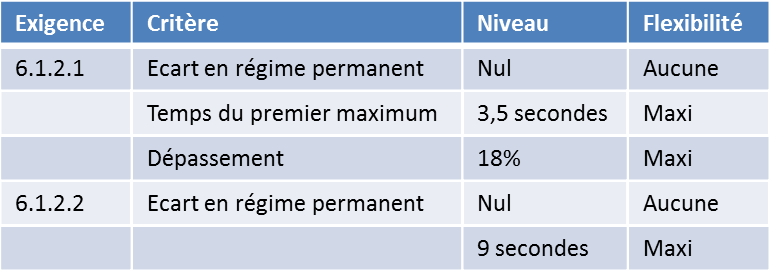
\includegraphics[width=.95\linewidth]{png/cdc}
\end{center}
\end{minipage}
\end{obj}



\subsection*{Modèle de connaissance du dispositif d’anti-enrayage}
\ifthenelse{\boolean{prof}}{}{
On suppose, pour la suite, que l’architecture de la boucle de régulation est
représentée sur la figure suivante où $\nu_c$ est la consigne de
glissement.

\begin{center}
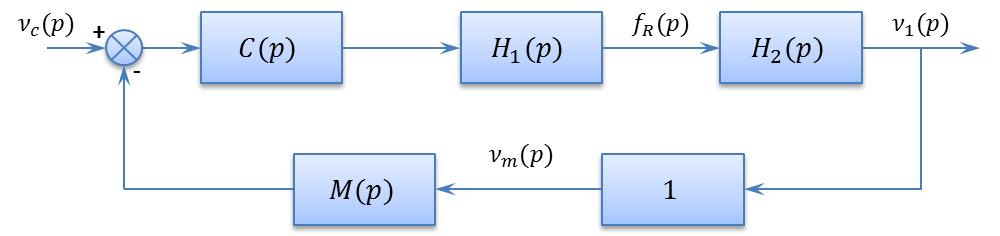
\includegraphics[width=.6\textwidth]{png/regul2.png}
\end{center}

\begin{itemize}
\item $H_1(p)$ : fonction de transfert de l’actionneur de freinage (vérin pneumatique
+ électrovalve) ;
\item $H_2(p)$ : fonction de transfert de la roue au freinage;
\item $C(p)$ : correcteur de la boucle de régulation;
\item $M(p)$ : fonction de transfert de la chaîne de mesure du glissement obtenu à
partir des vitesses $V_T$ et $V_R$, cette chaîne comporte un filtre destiné à limiter
l’impact des bruits de mesure ;
\item $\nu_m$ : glissement estimé à partir de $V_T$ et de $V_R$.
\end{itemize}
On adoptera pour la suite :
\begin{equation}
H_1(p)=\dfrac{2000}{\left(1+0,1p + 0,01 p^2 \right)}
\end{equation}


\begin{equation}
M(p)=\dfrac{1}{\left(1+0,05p \right)}
\end{equation}


\begin{equation}
\nu_1(t)+\dfrac{I\cdot V_{T_0}}{r^2Mgf'(\nu_0)}\dot{\nu_1}(t)=\dfrac{1}{Mgf'(\nu_0)}f_R(t)
\end{equation}

Les données numériques utilisées sont les suivantes :
$M = 8200\;kg$, $V_T= 200\; km\cdot h^{–1}$, $I/r^2=400\;kg$, $ g=10 m\cdot s^{–2}$

%Pour une vitesse $V_T=200\;km\cdot h^{-1}$, le cahier des charges est résumé par les %données
%du tableau 1 et les données numériques utilisées sont données ci-dessous.
%Enfin, les problèmes liés à l’évolution de la vitesse $V_T$ ne font pas l’objet de cette
%étude.




%
%\begin{center}
%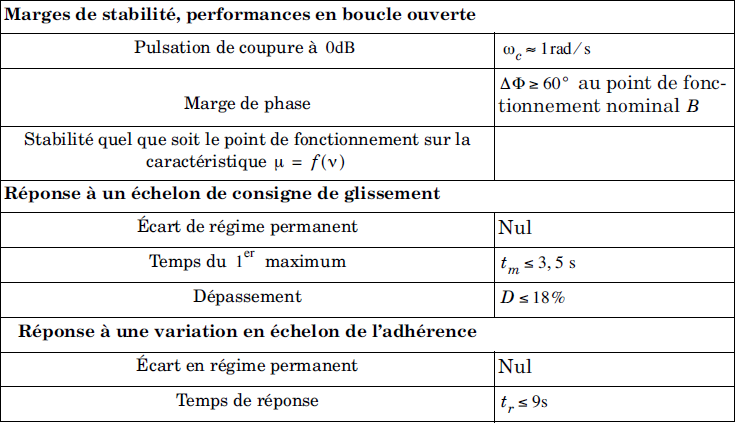
\includegraphics[width=.8\textwidth]{png/cfc.png}
%
%Cahier des charges de la boucle de régulation de glissement pour $V_T=200\;km\cdot h^{-1}$
%\end{center}

%\subsection{Analyse des réponses fréquentielles en boucle ouverte}

%\subsection{Synthèse du régulateur de la boucle de régulation}

}
\subsection*{Vérification du cahier des charges vis-à-vis de la consigne de glissement}

\ifthenelse{\boolean{prof}}{}{
Le correcteur de la boucle de régulation du dispositif d’anti-enrayage est de cette forme :
$$
C(p)=K_r\left( 1 + \dfrac{1}{T_i p} \right)
$$

L’objectif de cette partie
est de vérifier que le correcteur permet de satisfaire le cahier des charges.
Cette vérification concerne d’une part les performances vis-à-vis des variations
de la consigne de glissement : temps du 1\up{er} maximum, dépassement, écart
en régime permanent et d’autre part la réponse vis-à-vis des variations d’adhérence.
}

%\subparagraph{Question 1}
%\textit{Calculer la fonction de transfert $H_2(p)$ associée à la relation (3).}

\subparagraph{}
\textit{Mettre la relation (3) dans le domaine de Laplace et exprimer $H_2(p)$.}
\ifthenelse{\boolean{prof}}{
\begin{corrige}
$$
\nu_1(t)+\dfrac{I\cdot V_{T_0}}{r^2 M g f'(v_0)} \dfrac{\nu_1(t)}{dt} = \dfrac{1}{Mgf'(\nu_0)}f_R(t)
$$
 
$$
\Longleftrightarrow V_1(p)+p\dfrac{I\cdot V_{T_0}}{r^2 M g f'(v_0)} V_1(p) = \dfrac{1}{Mgf'(\nu_0)}F_R(p)
$$

On note :
$$
\alpha = \dfrac{I\cdot V_{T_0}}{r^2 M g f'(v_0)} \quad \beta = \dfrac{1}{Mgf'(\nu_0)}
$$

On a donc : 
$$
V_1(p)+\alpha p V_1(p) = \beta F_R(p)
$$

En conséquence :
$$
H_2(p) = \dfrac{ V_1(p)}{F_R(p)}=\dfrac{\beta}{1+\alpha p}
$$
\end{corrige}
}{}


\subparagraph{}
\textit{Calculer la fonction de transfert en boucle fermé du système. On la notera $F(p)$ : }
$$
F(p)=\dfrac{\nu_1(p)}{\nu_c(p)}
$$ 
\ifthenelse{\boolean{prof}}{
\begin{corrige}
Par définition, on a :
$$
F(p)=\dfrac{V_1(p)}{V_c(p)} = \dfrac{C(p) H_1(p) H_2(p)}{1+C(p) H_1(p) H_2(p)M(p)}
$$

En remplaçant les fonctions de transfert par leur expression, on obtient : 
$$
F(p) = \dfrac{\dfrac{K_rT_i p + K_r}{T_i p} \dfrac{2000}{1+0,1 p +0,01 p^2} \dfrac{\beta}{1+\alpha p}}{1+\dfrac{K_rT_i p + K_r}{T_i p} \dfrac{2000}{1+0,1 p +0,01 p^2} \dfrac{\beta}{1+\alpha p} \dfrac{1}{1+0,05p}}
$$


$$
F(p) = \dfrac{2000\cdot\beta \left( K_rT_i p + K_r\right)}{
\left(1+\alpha p\right)\left(1+0,1 p +0,01 p^2\right)T_i p+2000\cdot \beta \dfrac{K_rT_i p + K_r}{1+0,05p}
}
$$

Au final : 

$$
F(p) = \dfrac{2000\cdot\beta \left( K_rT_i p + K_r\right)\left(1+0,05p\right)}{
\left(1+0,05p\right)\left(1+\alpha p\right)\left(1+0,1 p +0,01 p^2\right)T_i p+2000\cdot \beta \left(K_rT_i p + K_r\right)}
$$
\end{corrige}
}{}


\subparagraph{}
\textit{Calculer l'écart statique du système.}

\ifthenelse{\boolean{prof}}{
\begin{corrige}
L'écart statique d'un système est calculée à l'aide d'une entrée échelon. 

Commençons par calculer la valeur finale atteinte par le système.

$$
V_c(p)=\dfrac{1}{p}
$$

$$
\lim\limits_{t\to +\infty}v_1(t)=\lim\limits_{p\to 0}pV_1(p)=\lim\limits_{p\to +0}pV_c(p)F(p)
$$

$$
F(p) = \dfrac{2000\cdot \beta \left( K_rT_i p + K_r\right)\left(1+0,05p\right)}{
\left(1+\alpha p\right)\left( K_rT_i p + K_r\right)\left(1+0,1 p +0,01 p^2\right)T_i p+2000\cdot \beta \left( K_rT_i p + K_r\right)
}
$$

et 
$$
pV_c(p) = 1
$$
On a donc 
$$
\lim\limits_{t\to +\infty}v_1(t)=\lim\limits_{p\to 0}F(p) = \dfrac{2000\cdot\beta K_r}{ 2000 \cdot \beta K_r  }=1
$$

L'entrée étant un échelon d'amplitude, l'écart statique est donc nul (1-1). Le système est donc précis.

\end{corrige}
}{}


Pour la suite, on adoptera la relation suivante :

$$
F(p)=\dfrac{\nu_1(p)}{\nu_c(p)}=\dfrac{K_f\left( 1+\tau_1 p\right)}{\left( 1+\tau_2 p\right)^2}
$$

\subparagraph{}
\textit{Donner la fonction de transfert associée à une entrée échelon.}

\ifthenelse{\boolean{prof}}{
\begin{corrige}
La fonction de transfert d'une fonction échelon dans le domaine de Laplace est la suivante :
$$
V_c(p)=\dfrac{1}{p}
$$

\end{corrige}
}{}



\subparagraph{}
\textit{Calculer la réponse temporelle du système pour une entrée indicielle (réponse à un échelon).}
\textit{Vous détaillerez les étapes permettant de calculer la décomposition en éléments simples.}
On donne pour cela :
$$
\mathcal{L}\left[ t^n e^{-at} \right] = \dfrac{n!}{(p+a)^{n+1}}
$$

\ifthenelse{\boolean{prof}}{
\begin{corrige}

À partir de la fonction $F(p)$ donnée on a donc : 
$$
V_1(p) = \dfrac{1}{p} \cdot \dfrac{\nu_1(p)}{\nu_c(p)}=\dfrac{K_f\left( 1+\tau_1 p\right)}{p\left( 1+\tau_2 p\right)^2}
$$

Il est donc possible de mettre $V_1(p)$ sous la forme : 
$$
V_1(p) = \dfrac{\alpha}{p}+\dfrac{\beta}{1+\tau_2 p}+\dfrac{\gamma}{(1+\tau_2 p)^2}
$$

En multipliant les deux expressions de $V_1(p)$ par $p$, on a :
$$
p\dfrac{K_f\left( 1+\tau_1 p\right)}{p\left( 1+\tau_2 p\right)^2} = 
p\dfrac{\alpha}{p}+p\dfrac{\beta}{1+\tau_2 p}+p\dfrac{\gamma}{(1+\tau_2 p)^2}
\Longleftrightarrow
\dfrac{K_f\left( 1+\tau_1 p\right)}{\left( 1+\tau_2 p\right)^2} = 
\alpha+p\dfrac{\beta}{1+\tau_2 p}+p\dfrac{\gamma}{(1+\tau_2 p)^2}
$$

En posant $p=0$, on a donc directement : 
$$
\alpha = K_f
$$

En multipliant les deux expressions de $V_1(p)$ par $\left(1+\tau_2 p\right)^2$, on a :
$$
\left(1+\tau_2 p\right)^2\dfrac{K_f\left( 1+\tau_1 p\right)}{p\left( 1+\tau_2 p\right)^2} = 
\left(1+\tau_2 p\right)^2\dfrac{\alpha}{p}+\left(1+\tau_2 p\right)^2\dfrac{\beta}{1+\tau_2 p}+\left(1+\tau_2 p\right)^2\dfrac{\gamma}{(1+\tau_2 p)^2}
$$
$$
\Longleftrightarrow
\dfrac{K_f\left( 1+\tau_1 p\right)}{p} = 
\left(1+\tau_2 p\right)^2\dfrac{\alpha}{p} + \beta  \left(1+\tau_2 p\right)
+\gamma
$$

En posant $p=\dfrac{-1}{\tau_2}$, on a donc directement : 
$$
\gamma = K_f\left( \tau_1 - \tau_2\right)
$$

Pour déterminer $\beta$, utilisons une valeur particulière. Calculons donc $V_1(1)$ avec les deux expressions de $V_1$ :
$$
V_1(1)=\dfrac{K_f\left(1+\tau_1\right)}{\left(1+\tau_2\right)^2} = K_f + \dfrac{\beta}{1+\tau_2}+\dfrac{K_f\left( \tau_1 - \tau_2\right)}{\left(1+\tau_2\right)^2}
$$

$$
\beta = -K_f \tau_2
$$
D'où 
$$
V_1(p) = \dfrac{K_f}{p}-\dfrac{K_f \tau_2}{1+\tau_2 p}+\dfrac{K_f\left(\tau_1 - \tau_2 \right)}{(1+\tau_2 p)^2}
$$

En utilisant la transformée de Laplace inverse, on obtient : 
$$
\nu_1(t)=\left(K_f  -K_f e^{-\dfrac{t}{\tau_2}}+\dfrac{K_f \left(\tau_1 - \tau_2 \right)}{\tau_2^2}te^{-\dfrac{t}{\tau_2}}\right) u(t)
$$


\end{corrige}
}{}


%$$
%\mathcal{L}\left[ e^{-at} \right] = \dfrac{1}{p+a}
%$$

\subparagraph{}
\textit{A partir de la réponse temporelle, donner une \textbf{méthode} permettant de calculer le premier dépassement.}
\ifthenelse{\boolean{prof}}{
\begin{corrige}
D'après la courbe on observe un seul dépassement $t_m$. Il est donc nécessaire de résoudre : 
$$
\dfrac{d\nu_1(t)}{dt}=0
$$

La valeur de $t_m$ donnera donc le temps auquel a lieu le maximum du dépassement.

En calculant alors $\nu_1(t_m)$, on obtient la valeur du dépassement.

Par le calcul, on obtient $t_m=3,3 s.$ et $\nu(t_m)=1,13$  soit un dépassement de 13\%.
\end{corrige}
}{}


\ifthenelse{\boolean{prof}}{}{
La courbe donnée par la réponse indicielle est donnée ci-dessous.
\begin{center}
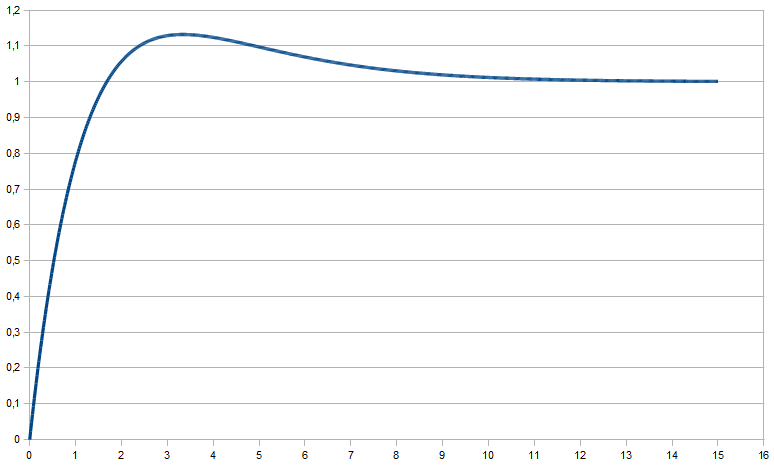
\includegraphics[width=.8\textwidth]{png/courb1.png}
\end{center}
}
\subparagraph{}
\textit{A partir de la courbe, donner : 
\begin{itemize}
\item le temps du premier dépassement;
\item le dépassement en pourcentage.
\end{itemize}
Vous indiquerez les relevés effectués sur la courbe donnée en fin de sujet.
}

\ifthenelse{\boolean{prof}}{
\begin{corrige}
Le lecture de la courbe confirme les valeurs données ci-dessus :
\begin{itemize}
\item le temps du premier dépassement : 3,3 s.
\item le dépassement en pourcentage : 13\%
\end{itemize}

\begin{center}
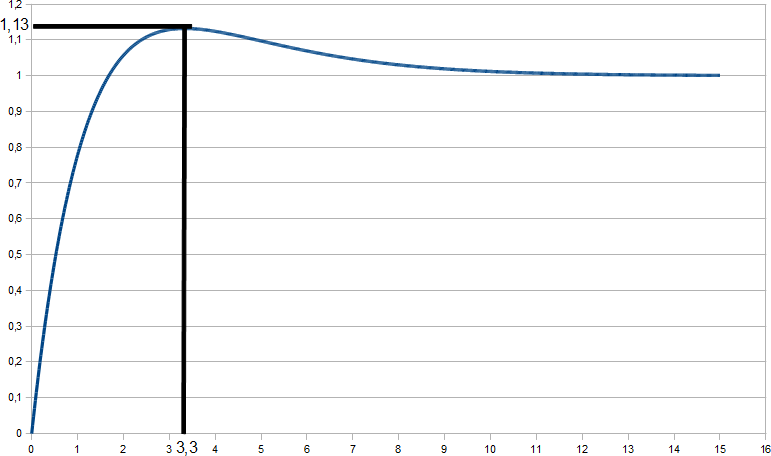
\includegraphics[width=.5\textwidth]{png/courb1_Cor.png}
\end{center}

\end{corrige}
}{}

\subparagraph{}
\textit{\'A partir de ces mesures, peut-on dire que le cahier des charges est vérifié ?}

\ifthenelse{\boolean{prof}}{
\begin{corrige}
Le temps du premier maximum est inférieur à 3,5 s. Le dépassement est de 13\% ce qui est inférieur à 18\%. Le cahier des charges est donc vérifié.

\end{corrige}
}{}


\subsection*{Analyse des performances temporelles en réponse à des variations d'adhérence}

\ifthenelse{\boolean{prof}}{}{
La variation d'adhérence peut être modélisée en première approximation comme une force perturbatrice externe additive $f_{ext}$. On admet que cette modélisation conduit au schéma bloc représenté sur la figure 14.

On se propose dans
cette partie d’évaluer les performances de la chaîne de régulation de freinage vis à-
vis de cette perturbation.

\begin{center}
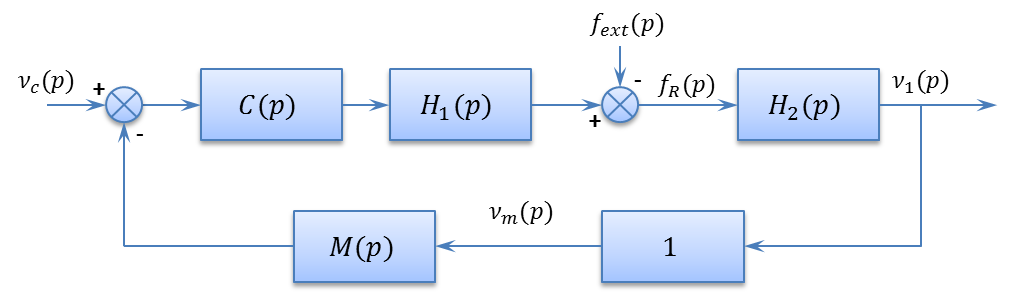
\includegraphics[width=.6\textwidth]{png/regul_perturb2.png}
\end{center}
}

\subparagraph{}
\textit{En utilisant le théorème de superposition et donc en tenant compte de la perturbation, calculer $\nu_1(p)$ en fonction de $F_{ext}(p)$ et $\nu_c(p)$.}

\ifthenelse{\boolean{prof}}{
\begin{corrige}
En considérant que $F_{ext}(p)$ est nul, on a :
$$
\dfrac{V_1(p)}{V_c(p)}=\dfrac{C(p) H_1(p) H_2(p) }{1+ C(p) H_1(p) H_2(p) M(p)}
$$

En considérant que $V_C(p)$ est nul, on a :
$$
\dfrac{V_1(p)}{F_{ext}(p)}=\dfrac{H_2(p) }{1+ C(p) H_1(p) H_2(p) M(p)}
$$

Au final, (attention au signe moins du comparateur de la perturbation) :
$$
V_1(p)=V_c(p)\cdot \dfrac{C(p) H_1(p) H_2(p) }{1+ C(p) H_1(p) H_2(p) M(p)} - F_{ext}(p) \dfrac{H_2(p) }{1+ C(p) H_1(p) H_2(p) M(p)}
$$

\end{corrige}
}{}


\subparagraph{}
\textit{Quel sera l'écart statique si le système est sollicité par une entrée $\nu_c(p)$ indicielle et une perturbation $f_{ext}(p)$ indicielle.}

\ifthenelse{\boolean{prof}}{
\begin{corrige}
\end{corrige}
}{}



\ifthenelse{\boolean{prof}}{}{
On donne le tracé de la réponse temporelle à une variation en échelon de l'adhérence.

\begin{center}
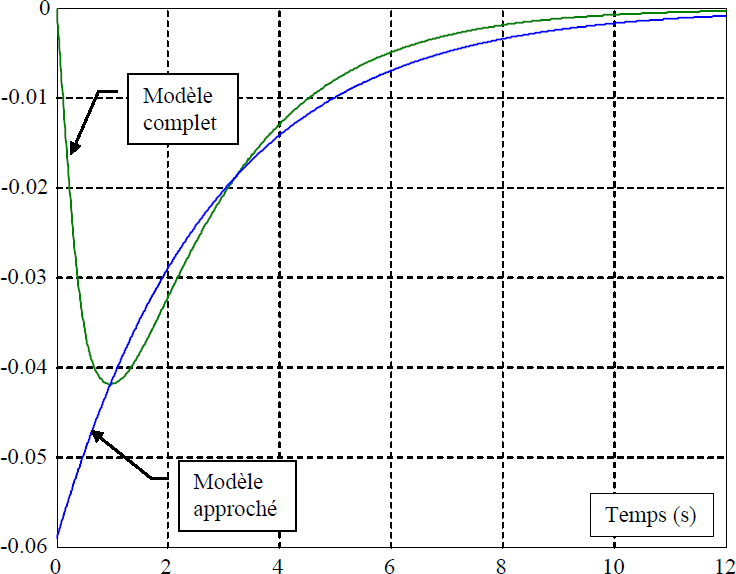
\includegraphics[width=.6\textwidth]{png/courb2.png}
\end{center}
Grâce au modèle approché, il est possible de modéliser le fonctionnement du système par une fonction de transfert du premier ordre. Une fonction de transfert du premier ordre est donnée par la relation suivante :
$$
G(p)=\dfrac{K_G}{1+\tau_G p}
$$
}

\subparagraph{}
\textit{A partir de la lecture de la courbe, donner la constante de temps $\tau_G$ du système par la méthode de votre choix.
Indiquer vos relevés sur les courbes en fin de sujet.}

\ifthenelse{\boolean{prof}}{
\begin{corrige}

3 méthodes permettent de mesurer $\tau_G$ pour un système du premier ordre:
\begin{itemize}
\item la tangente à l'origine coupe la valeur finale en $t=\tau_G$;
\item à 63\% de la valeur finale, on a $t=\tau_G$;
\item à 95\% de la valeur finale, on a  $t=3\tau_G$.
\end{itemize}

La lecture de la question suivante nous indique qu'il vaut peut être mieux utiliser la troisième méthode.

On a donc $\tau_G = 2,66\;s.$ 
\begin{center}
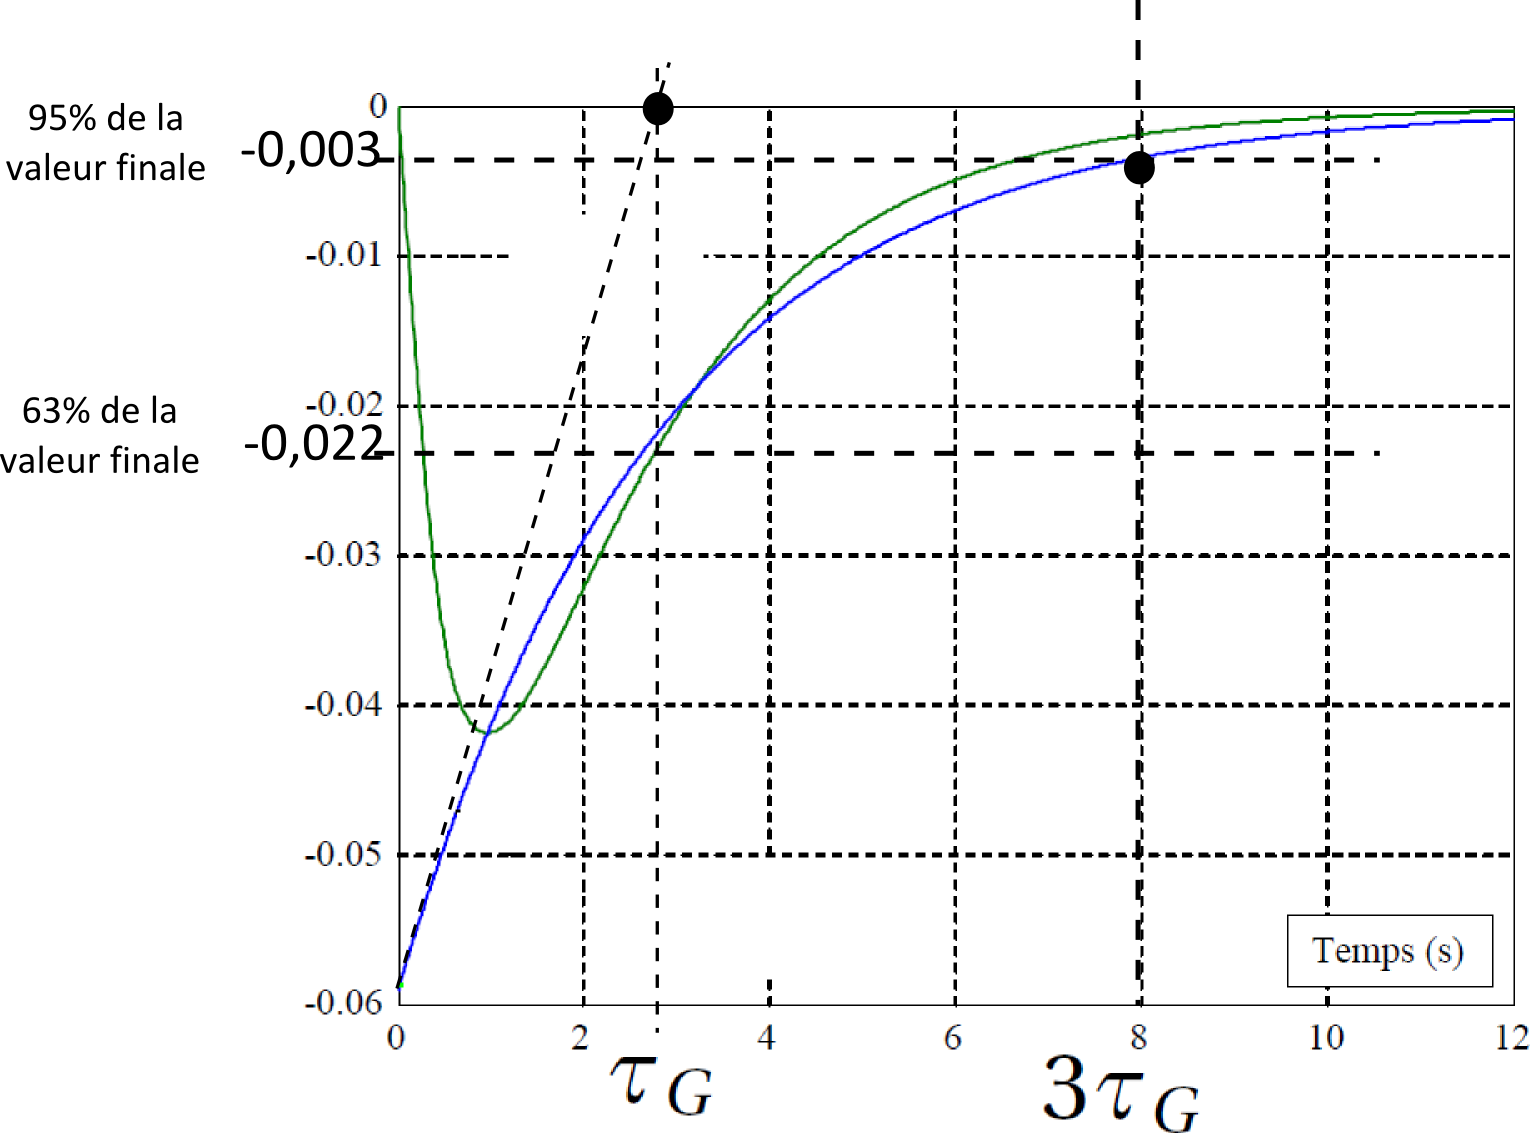
\includegraphics[width=.5\textwidth]{png/courb2_Cor.png}
\end{center}


\end{corrige}
}{}

\subparagraph{}
\textit{A partir de la lecture de la courbe, donner le temps de réponse à 5\%.}

\ifthenelse{\boolean{prof}}{
\begin{corrige}
Le temps de réponse à 5\% de la valeur finale est de 8 secondes.

\end{corrige}
}{}

\subparagraph{}
\textit{Conclure sur les performances obtenues vis-à-vis des exigences du cahier des charges à des variations de l'adhérence.}

\ifthenelse{\boolean{prof}}{
\begin{corrige}

D'après le cahier des charges, le temps de réponse doit être inférieur à 9s.
Le temps de réponse est de 8 secondes. Le cahier des charges est vérifié.


\end{corrige}
}{}

\ifthenelse{\boolean{prof}}{}{

\newpage

\begin{center}
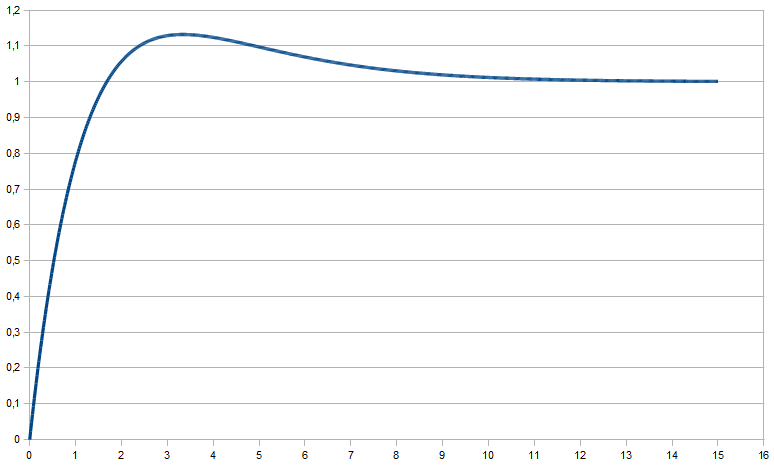
\includegraphics[width=.8\textwidth]{png/courb1.png}
\end{center}

\vspace{2cm}

\begin{center}
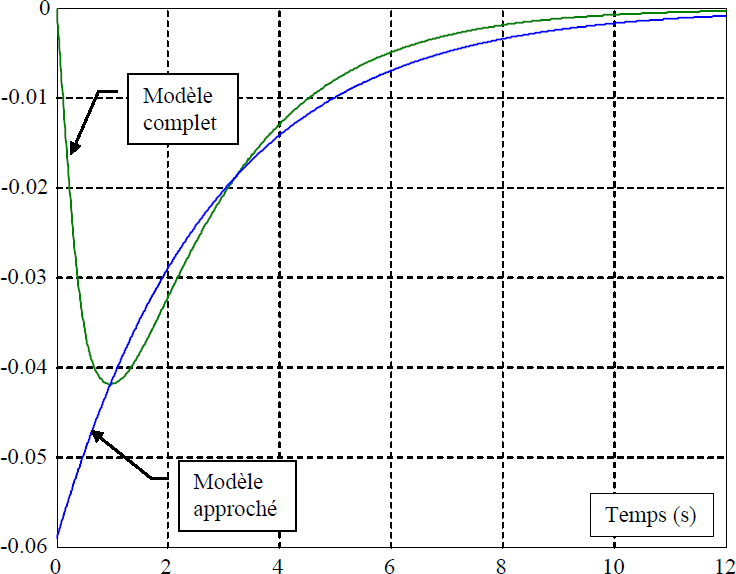
\includegraphics[width=.8\textwidth]{png/courb2.png}
\end{center}




%\subparagraph{}
%\textit{}
%\ifthenelse{\boolean{prof}}{
%\begin{corrige}
%\end{corrige}
%}{}

\newpage


\section*{Compléments}

\noindent\begin{minipage}[t]{.48\linewidth}
\subsection*{Calcul théorique de l'écart statique}
\begin{methode}

\textbf{Méthode 1 }

Dans le cas où $e(t)$ et $s(t)$ sont des grandeurs de même nature physique (même unité), l'écart statique peut être calculé ainsi :
$$
\varepsilon_s = \lim\limits_{t\to +\infty} |s(t)-e(t)|
$$


\textbf{Méthode 2}

On peut montrer que :
$$
\varepsilon_s = \lim\limits_{t\to +\infty} \varepsilon(t)
$$

Par passage au théorème de la valeur finale on a donc : 
$$
\varepsilon_s = \lim\limits_{t\to +\infty} \varepsilon(t)=  \lim\limits_{t\to 0} p \varepsilon(p)
$$
\end{methode}

\end{minipage}\hfill
\begin{minipage}[t]{.48\linewidth}
\subsection*{Détermination graphique de l'écart statique}

\vspace{1cm}

\begin{center}
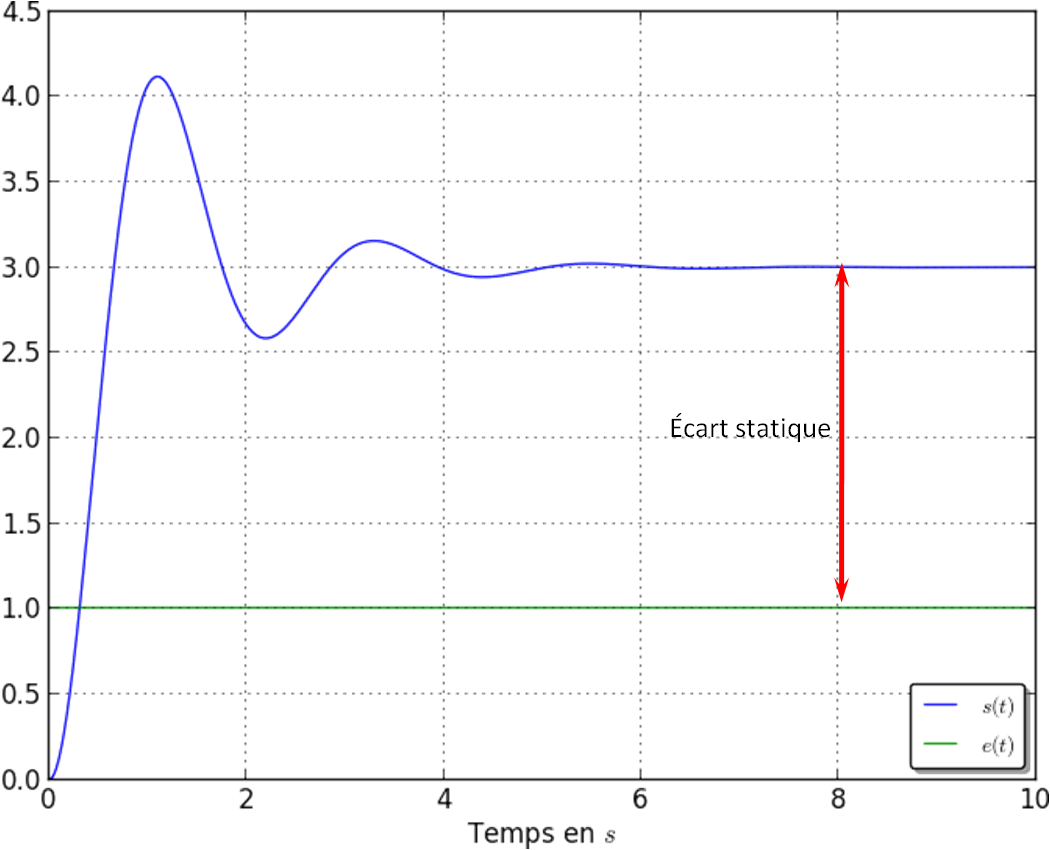
\includegraphics[width=\textwidth]{png/EcartStatique.png}
\end{center}

L'entrée et la sortie doivent être de même nature.
\end{minipage}


%On donne un système asservi avec uns structure classique :
%\begin{center}
%%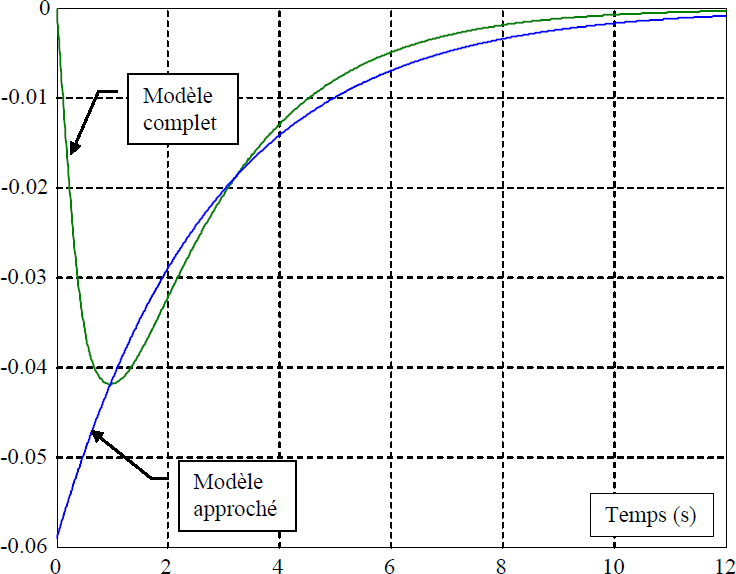
\includegraphics[width=.8\textwidth]{png/courb2.png}
%\end{center}



\subsection*{Détermination graphique du temps de réponse à 5\%}

\begin{center}
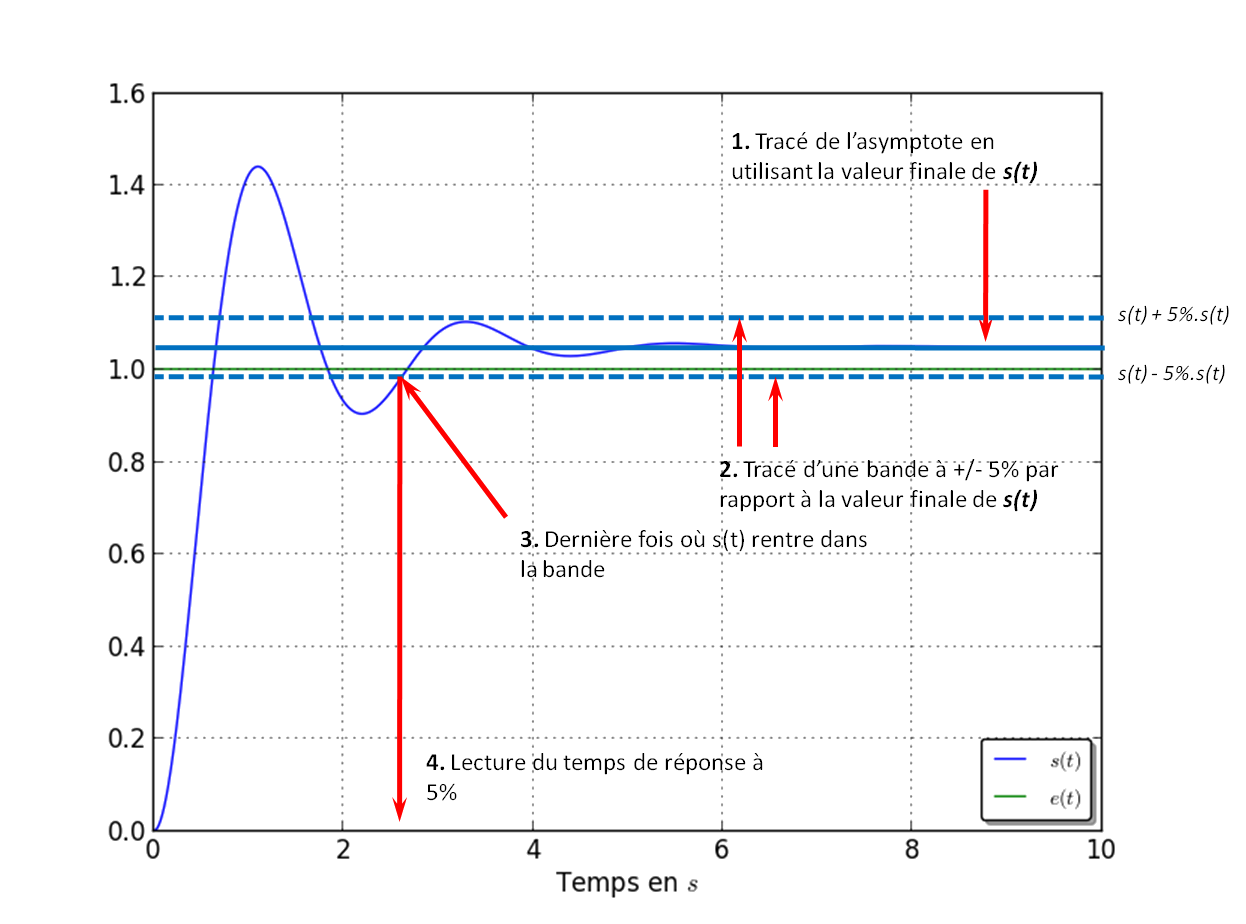
\includegraphics[width=.8\textwidth]{png/tr5.png}
\end{center}

\subsection*{Dépassement}

Le premier dépassement s'exprime ainsi (en pourcentage) :$D_{1\%}=\dfrac{\Delta_1}{\Delta}$.


\subsection*{Détermination de la constante de temps pour un système assimilable à un premier ordre}
\vspace{.5cm}

L'allure de la réponse indicielle d'un système d'ordre 1 est donné sur la figure suivante. Il existe 3 caractéristiques qui permettent de les identifier : 
\begin{itemize}
\item une tangente non nulle à l'origine;
\item pas de dépassement;
\item une tangente horizontale en l'infini.
\end{itemize}

\noindent\begin{minipage}[c]{.47\linewidth}
\begin{methode}
On note $\tau$ la constante de temps d'un système d'ordre 1. $\tau$ peut être déterminé de trois façons différentes :
\begin{enumerate}
\item On trace l'asymptote de la courbe lorsque $t$ tend vers l'infini et la tangente à l'origine. L'abscisse de l'intersection est $\tau$.
\item \'A 95\% de la valeur finale, le temps mesuré vaut 3$\tau$.
\item \'A 63\% de la valeur finale, le temps mesuré vaut $\tau$.
\end{enumerate}
\end{methode}
\end{minipage}\hfill
\begin{minipage}[c]{.47\linewidth}
\begin{center}
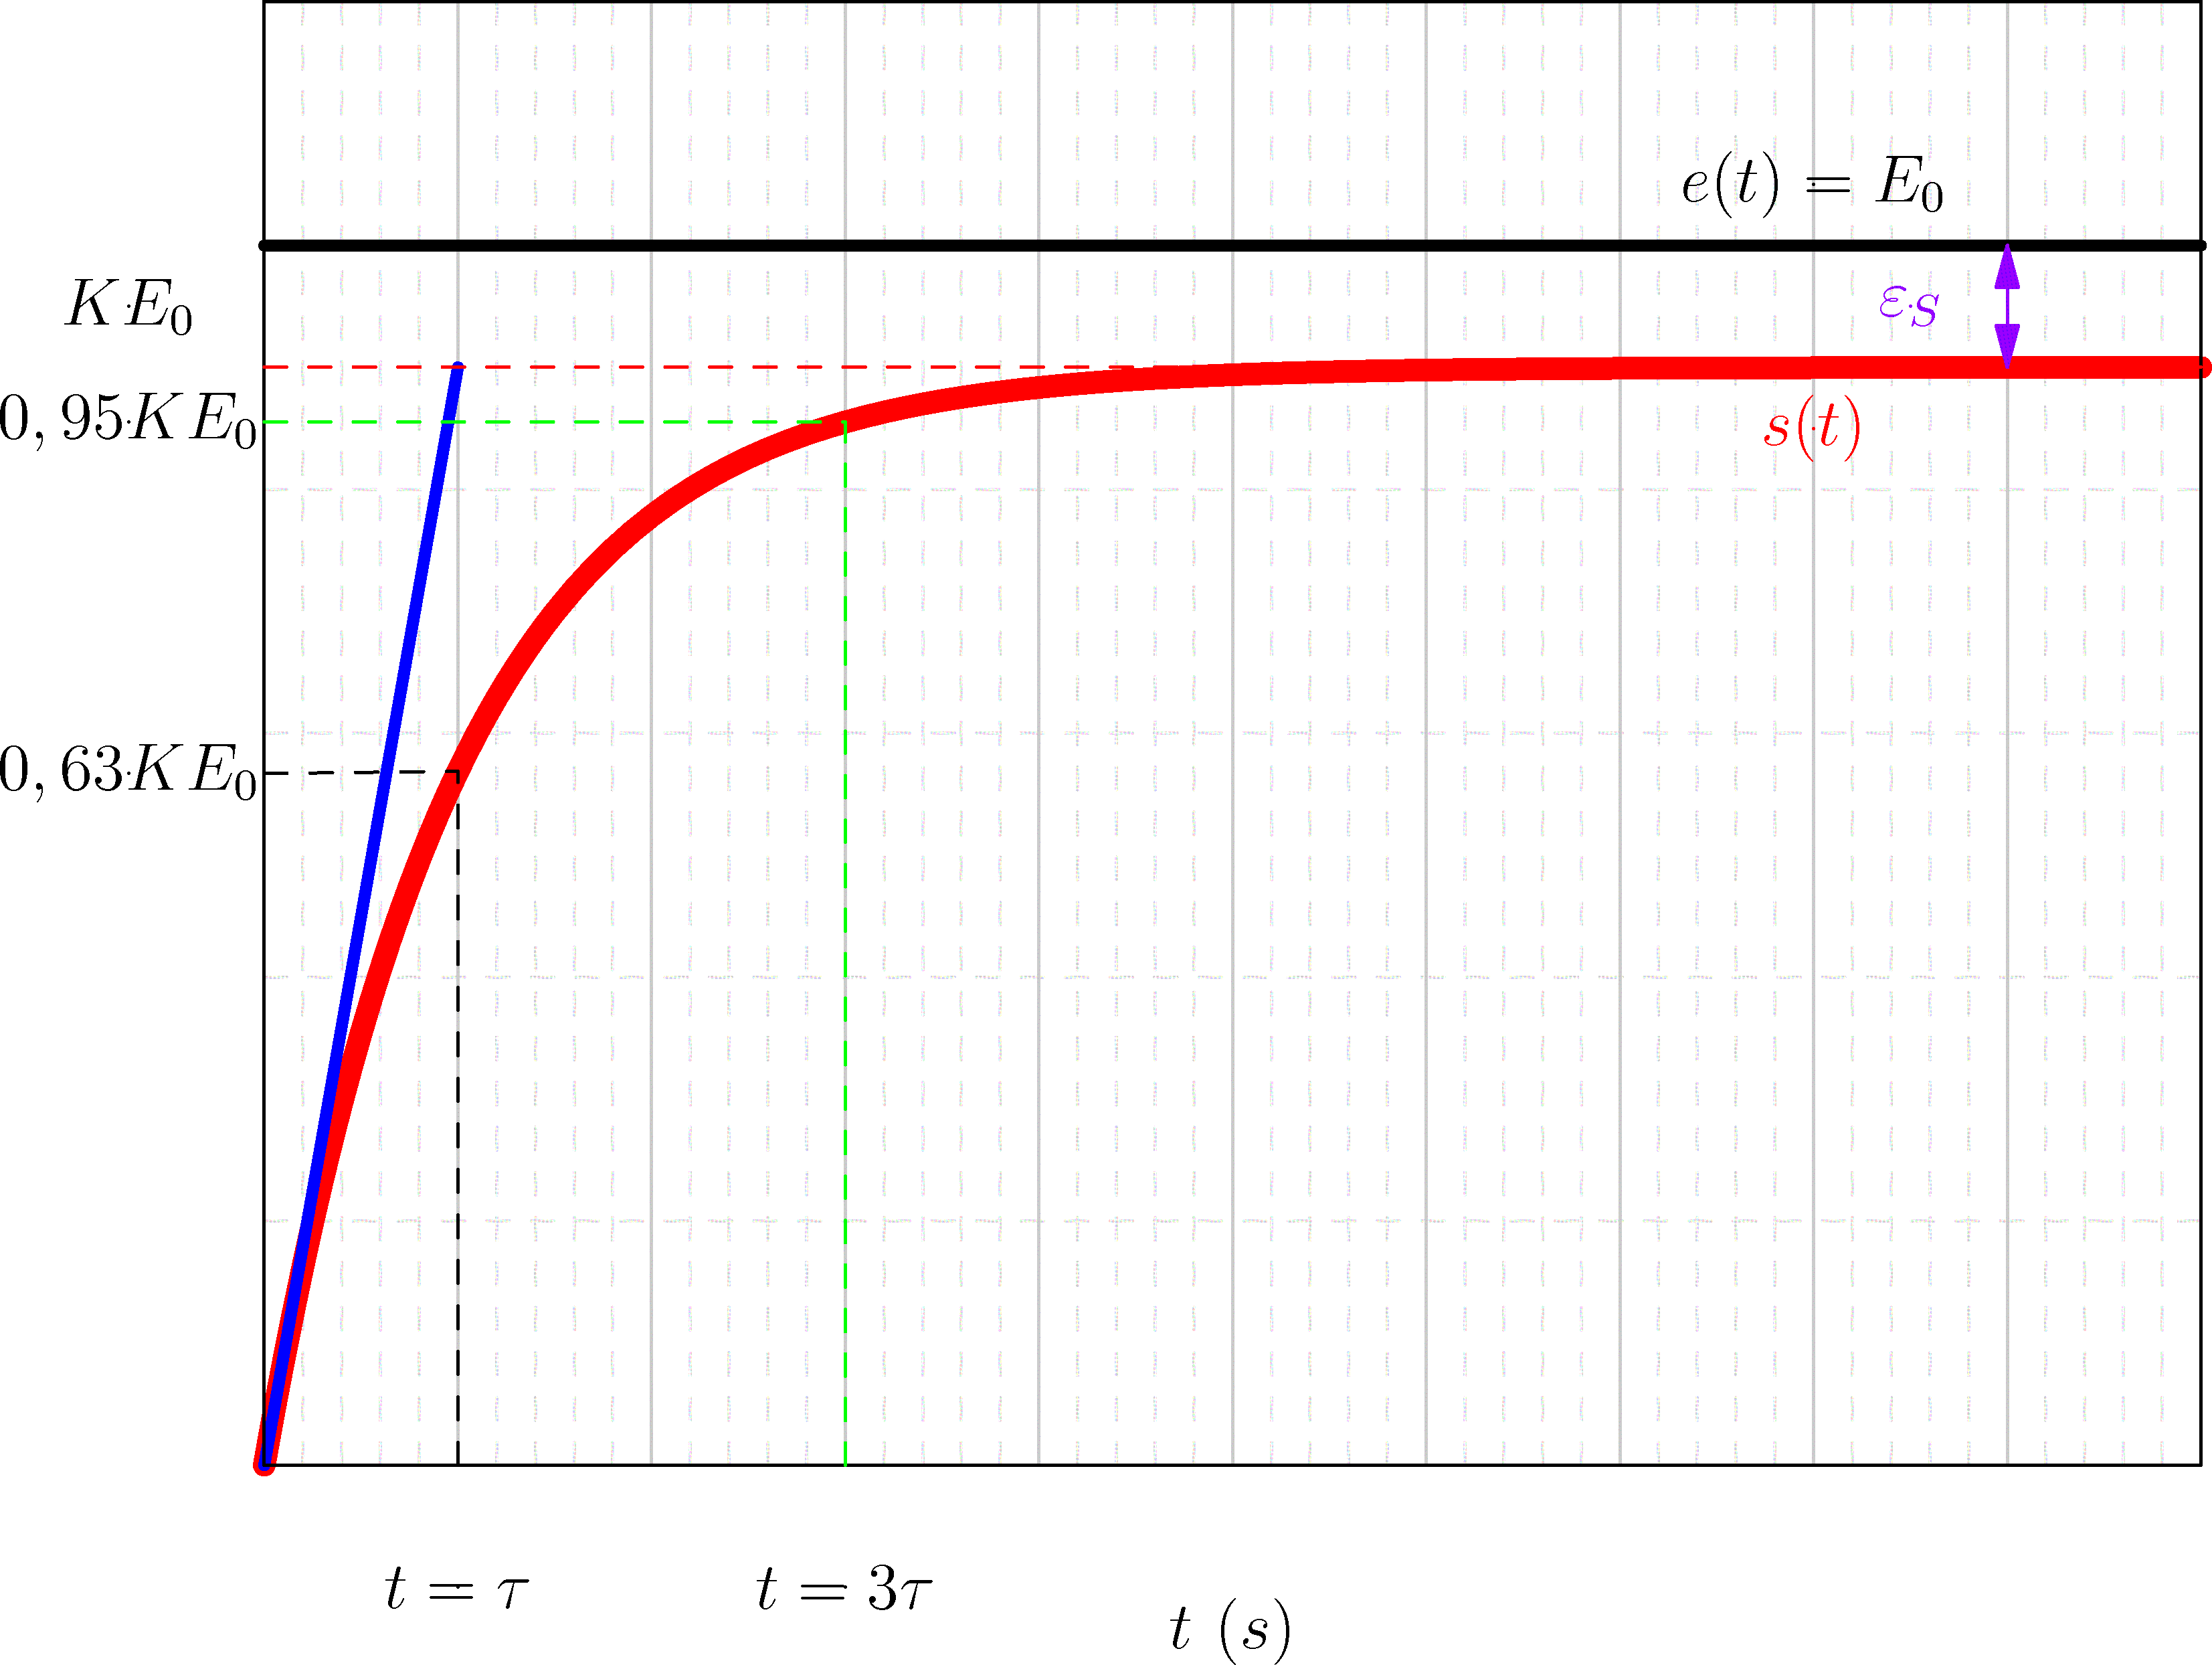
\includegraphics[width=\textwidth]{png/ordre1_echelon.png}
\end{center}
\end{minipage}
}

\end{document}
